% answers.tex —— 2004 年·普通高等学校招生考试·湖北卷·理科 · 参考答案与详细解析片段
% 由 tools/generate_projects.py 依来源总账自 2004/2004_数学真题_湖北理科_试题.md + 2004/2004_数学真题_湖北理科_解析正文.md + 2004/2004_数学真题_湖北理科_答案要点.md 生成，勿手改（改源 MD 后重跑）


\begin{gktip}
固定源 PDF 为印刷页码 170–171 的两页题面，不附官方答案。以下解析均依据固定源独立推导复算；各题配图在 LaTeX 工程中均以 TikZ 纯矢量重绘。
\end{gktip}

\begin{answer}
\gksolhead{1}{}

\textbf{题目}：

与直线 $2x - y + 4 = 0$ 平行的抛物线 $y = x^2$ 的切线方程是\mbox{（　　）}

\begin{gkopts}(4)
\task A．$2x - y + 3 = 0$
\task B．$2x - y - 3 = 0$
\task C．$2x - y + 1 = 0$
\task D．$2x - y - 1 = 0$
\end{gkopts}

\Needspace{4\baselineskip}
\textbf{解析}

\Needspace{5\baselineskip}
已知抛物线方程为 $y = x^2$，对其求导得：
\nopagebreak[4]
\[
y' = 2x.
\]
所求切线与直线 $2x - y + 4 = 0$（即 $y = 2x + 4$）平行，故切线的斜率 $k = 2$．
\Needspace{5\baselineskip}
令导数等于切线斜率：
\nopagebreak[4]
\[
2x = 2 \implies x = 1.
\]
将 $x = 1$ 代入抛物线方程得切点坐标为 $(1, 1)$．
\Needspace{5\baselineskip}
由点斜式写出切线方程：
\nopagebreak[4]
\[
y - 1 = 2(x - 1) \implies y = 2x - 1 \implies 2x - y - 1 = 0.
\]
故选 D．

\gkanswer{答案：D}

\end{answer}
\begin{answer}
\gksolhead{2}{}

\textbf{题目}：

复数 $\dfrac{(-1 + \sqrt{3}\mathrm{i})^5}{1 + \sqrt{3}\mathrm{i}}$ 的值是\mbox{（　　）}

\begin{gkopts}(1)
\task A．$-16$
\task B．$16$
\task C．$-\dfrac{1}{4}$
\task D．$\dfrac{1}{4} - \dfrac{\sqrt{3}}{4}\mathrm{i}$
\end{gkopts}

\Needspace{4\baselineskip}
\textbf{解析}

\Needspace{5\baselineskip}
将分子与分母分别化为三角形式或指数形式：
\nopagebreak[4]
\[
-1 + \sqrt{3}\mathrm{i} = 2\left(-\frac{1}{2} + \frac{\sqrt{3}}{2}\mathrm{i}\right) = 2\mathrm{e}^{\mathrm{i}\frac{2\pi}{3}}.
\]
\Needspace{5\baselineskip}
对其进行 $5$ 次方运算：
\nopagebreak[4]
\[
(-1 + \sqrt{3}\mathrm{i})^5 = 2^5 \mathrm{e}^{\mathrm{i}\frac{10\pi}{3}} = 32 \mathrm{e}^{\mathrm{i}\frac{4\pi}{3}} = 32\left(-\frac{1}{2} - \frac{\sqrt{3}}{2}\mathrm{i}\right) = -16(1 + \sqrt{3}\mathrm{i}).
\]
\Needspace{5\baselineskip}
因此：
\nopagebreak[4]
\[
\frac{(-1 + \sqrt{3}\mathrm{i})^5}{1 + \sqrt{3}\mathrm{i}} = \frac{-16(1 + \sqrt{3}\mathrm{i})}{1 + \sqrt{3}\mathrm{i}} = -16.
\]
故选 A．

\gkanswer{答案：A}

\end{answer}
\begin{answer}
\gksolhead{3}{}

\textbf{题目}：

已知 $f\left(\dfrac{1 - x}{1 + x}\right) = \dfrac{1 - x^2}{1 + x^2}$，则 $f(x)$ 的解析式可取为\mbox{（　　）}

\begin{gkopts}(2)
\task A．$\dfrac{x}{1 + x^2}$
\task B．$-\dfrac{2x}{1 + x^2}$
\task C．$\dfrac{2x}{1 + x^2}$
\task D．$-\dfrac{x}{1 + x^2}$
\end{gkopts}

\Needspace{4\baselineskip}
\textbf{解析}

设 $t = \dfrac{1 - x}{1 + x}$（$t \neq -1$）．
\Needspace{5\baselineskip}
两边同乘以 $1 + x$ 得：
\nopagebreak[4]
\[
t(1 + x) = 1 - x \implies t + tx = 1 - x \implies (t + 1)x = 1 - t \implies x = \frac{1 - t}{1 + t}.
\]
\Needspace{5\baselineskip}
将 $x = \dfrac{1 - t}{1 + t}$ 代入原函数右端的分子与分母：
\nopagebreak[4]
\[
1 - x^2 = 1 - \left(\frac{1 - t}{1 + t}\right)^2 = \frac{(1 + t)^2 - (1 - t)^2}{(1 + t)^2} = \frac{4t}{(1 + t)^2},
\]
\nopagebreak[4]
\[
1 + x^2 = 1 + \left(\frac{1 - t}{1 + t}\right)^2 = \frac{(1 + t)^2 + (1 - t)^2}{(1 + t)^2} = \frac{2(1 + t^2)}{(1 + t)^2}.
\]
\Needspace{5\baselineskip}
因此：
\nopagebreak[4]
\[
f(t) = \frac{1 - x^2}{1 + x^2} = \frac{\dfrac{4t}{(1 + t)^2}}{\dfrac{2(1 + t^2)}{(1 + t)^2}} = \frac{2t}{1 + t^2}.
\]
改换自变量符号得 $f(x) = \dfrac{2x}{1 + x^2}$．
故选 C．

\gkanswer{答案：C}

\end{answer}
\begin{answer}
\gksolhead{4}{}

\textbf{题目}：

已知 $\vec{a}, \vec{b}, \vec{c}$ 为非零的平面向量．甲：$\vec{a} \cdot \vec{b} = \vec{a} \cdot \vec{c}$，乙：$\vec{b} = \vec{c}$，则\mbox{（　　）}

\begin{gkopts}(2)
\task A．甲是乙的充分条件但不是必要条件
\task B．甲是乙的必要条件但不是充分条件
\task C．甲是乙的充要条件
\task D．甲既不是乙的充分条件也不是乙的必要条件
\end{gkopts}

\Needspace{4\baselineskip}
\textbf{解析}

若乙成立，即 $\vec{b} = \vec{c}$，由向量数量积的唯一定义，显然有 $\vec{a} \cdot \vec{b} = \vec{a} \cdot \vec{c}$（甲成立）．故乙可以推出甲，甲是乙的必要条件；
\Needspace{5\baselineskip}
若甲成立，即 $\vec{a} \cdot \vec{b} = \vec{a} \cdot \vec{c}$，移项提取公因式得：
\nopagebreak[4]
\[
\vec{a} \cdot (\vec{b} - \vec{c}) = 0.
\]
由于 $\vec{a}$ 为非零平面向量，只需差向量 $\vec{b} - \vec{c}$ 与 $\vec{a}$ 正交（即 $\vec{a} \perp (\vec{b} - \vec{c})$）即可，并不一定有 $\vec{b} - \vec{c} = \vec{0}$（即 $\vec{b} = \vec{c}$）．例如取 $\vec{a} = (1, 0)$，$\vec{b} = (1, 1)$，$\vec{c} = (1, 2)$，有 $\vec{a} \cdot \vec{b} = 1 = \vec{a} \cdot \vec{c}$，但 $\vec{b} \neq \vec{c}$．故甲不能推出乙，甲不是乙的充分条件．
综上，甲是乙的必要条件但不是充分条件．
故选 B．

\gkanswer{答案：B}

\end{answer}
\begin{answer}
\gksolhead{5}{}

\textbf{题目}：

若 $\dfrac{1}{a} < \dfrac{1}{b} < 0$，则下列不等式① $a + b < ab$；② $|a| > |b|$；③ $a < b$；④ $\dfrac{b}{a} + \dfrac{a}{b} > 2$ 中，正确的不等式有\mbox{（　　）}

\begin{gkopts}(4)
\task A．$1$ 个
\task B．$2$ 个
\task C．$3$ 个
\task D．$4$ 个
\end{gkopts}

\Needspace{4\baselineskip}
\textbf{解析}

已知 $\dfrac{1}{a} < \dfrac{1}{b} < 0$．
因为两数均为负数，取倒数后改变不等号方向，得 $a > b$ 且 $0 > a > b$．
逐一检验题干中给出的四个不等式：
\begin{itemize}
\item 对于① $a + b < ab$：因为 $a < 0, b < 0$，两负数之和为负数，即 $a + b < 0$；而同号相乘为正数，即 $ab > 0$．负数严格小于正数，因此 $a + b < ab$ 恒成立，① 正确；
\item 对于② $|a| > |b|$：由 $0 > a > b$ 可知 $|a| = -a$，$|b| = -b$．两边同乘 $-1$ 得 $-a < -b$，即 $|a| < |b|$（例如取 $a = -1, b = -2$，有 $|a| = 1 < 2 = |b|$），故② 错误；
\item 对于③ $a < b$：由已知严格推得 $a > b$，故③ 错误；
\item 对于④ $\dfrac{b}{a} + \dfrac{a}{b} > 2$：因为 $a$ 与 $b$ 同为负数且 $a \neq b$，所以 $\dfrac{b}{a} > 0$，$\dfrac{a}{b} > 0$，且 $\dfrac{b}{a} \neq 1$．根据基本不等式，对任意正且不相等的两实数，其和严格大于 $2$，即 $\dfrac{b}{a} + \dfrac{a}{b} > 2$ 恒成立，故④ 正确．
\end{itemize}
综上，正确的不等式共有 ① 和 ④ 两个．
故选 B．

\gkanswer{答案：B}

\end{answer}
\begin{answer}
\gksolhead{6}{}

\textbf{题目}：

已知椭圆 $\dfrac{x^2}{16} + \dfrac{y^2}{9} = 1$ 的左、右焦点分别为 $F_1$、$F_2$，点 $P$ 在椭圆上，若 $P$、$F_1$、$F_2$ 是一个直角三角形的三个顶点，则点 $P$ 到 $x$ 轴的距离为\mbox{（　　）}

\begin{gkopts}(2)
\task A．$\dfrac{9}{5}$
\task B．$3$
\task C．$\dfrac{9\sqrt{7}}{7}$
\task D．$\dfrac{9}{4}$
\end{gkopts}

\Needspace{4\baselineskip}
\textbf{解析}

椭圆方程为 $\dfrac{x^2}{16} + \dfrac{y^2}{9} = 1$，对应参数 $a = 4, b = 3, c = \sqrt{a^2 - b^2} = \sqrt{16 - 9} = \sqrt{7}$．
左、右焦点分别为 $F_1(-\sqrt{7}, 0), F_2(\sqrt{7}, 0)$，焦点在 $x$ 轴上，焦距 $|F_1F_2| = 2\sqrt{7}$．
点 $P$ 在椭圆上，且 $P, F_1, F_2$ 构成直角三角形：
\begin{itemize}
\item 情形一：直角顶点为焦点（$F_1$ 或 $F_2$），即 $PF_1 \perp F_1F_2$ 或 $PF_2 \perp F_1F_2$．
\end{itemize}
  此时点 $P$ 的横坐标为 $x = \pm c = \pm \sqrt{7}$（即通径端点）．
\Needspace{5\baselineskip}
  代入椭圆方程：
\nopagebreak[4]
\[
\frac{7}{16} + \frac{y^2}{9} = 1 \implies \frac{y^2}{9} = \frac{9}{16} \implies y^2 = \frac{81}{16} \implies |y| = \frac{9}{4}.
\]
  此时点 $P$ 到 $x$ 轴的距离即为 $|y| = \dfrac{9}{4}$；
\begin{itemize}
\item 情形二：直角顶点为点 $P$，即 $\angle F_1PF_2 = 90^\circ$．
\end{itemize}
  在 $\mathrm{Rt}\triangle PF_1F_2$ 中，$|PF_1|^2 + |PF_2|^2 = |F_1F_2|^2 = (2c)^2 = 28$．
  由椭圆定义，$|PF_1| + |PF_2| = 2a = 8$．
\Needspace{5\baselineskip}
  两边平方得：
\nopagebreak[4]
\[
(|PF_1| + |PF_2|)^2 = |PF_1|^2 + |PF_2|^2 + 2|PF_1||PF_2| = 64,
\]
\nopagebreak[4]
\[
28 + 2|PF_1||PF_2| = 64 \implies |PF_1||PF_2| = 18.
\]
\Needspace{5\baselineskip}
  由三角形面积公式：
\nopagebreak[4]
\[
S = \frac{1}{2}|PF_1||PF_2| = 9 = \frac{1}{2}|F_1F_2| \cdot |y| = \sqrt{7}|y| \implies |y| = \frac{9}{\sqrt{7}} = \frac{9\sqrt{7}}{7}.
\]
  但注意椭圆上点的纵坐标范围为 $|y| \leqslant b = 3 = \sqrt{9}$，而 $\dfrac{9\sqrt{7}}{7} = \sqrt{\dfrac{81}{7}} \approx \sqrt{11.57} > 3$，超出了椭圆的有界范围（事实上，由于 $b = 3 > \sqrt{7} = c$，短轴端点对焦点的张角满足 $\tan\theta = \dfrac{c}{b} = \dfrac{\sqrt{7}}{3} < 1 \implies 2\theta < 90^\circ$，椭圆上任意点对两焦点的张角均严格小于 $90^\circ$，故直角不可能在点 $P$ 处取得）．
因此直角顶点只能为焦点，点 $P$ 到 $x$ 轴的距离为 $\dfrac{9}{4}$．
故选 D．

\gkanswer{答案：D}

\end{answer}
\begin{answer}
\gksolhead{7}{}

\textbf{题目}：

函数 $f(x) = a^x + \log_a (x + 1)$ 在 $[0, 1]$ 上的最大值与最小值之和为 $a$，则 $a$ 的值为\mbox{（　　）}

\begin{gkopts}(4)
\task A．$\dfrac{1}{4}$
\task B．$\dfrac{1}{2}$
\task C．$2$
\task D．$4$
\end{gkopts}

\Needspace{4\baselineskip}
\textbf{解析}

函数为 $f(x) = a^x + \log_a (x + 1)$，定义域包含 $[0, 1]$，其中底数 $a > 0$ 且 $a \neq 1$．
由于函数 $y_1 = a^x$ 与 $y_2 = \log_a(x+1)$ 具有相同的单调性：
\begin{itemize}
\item 当 $a > 1$ 时，$y_1$ 与 $y_2$ 在 $[0, 1]$ 上均单调递增，故 $f(x)$ 单调递增；
\item 当 $0 < a < 1$ 时，$y_1$ 与 $y_2$ 在 $[0, 1]$ 上均单调递减，故 $f(x)$ 单调递减．
\end{itemize}
无论哪种情况，$f(x)$ 在区间 $[0, 1]$ 上的最大值与最小值必定分别在端点 $x = 0$ 和 $x = 1$ 处取得．
\Needspace{5\baselineskip}
因此，最大值与最小值之和为：
\nopagebreak[4]
\[
f(0) + f(1) = (a^0 + \log_a 1) + (a^1 + \log_a 2) = (1 + 0) + (a + \log_a 2) = 1 + a + \log_a 2.
\]
\Needspace{5\baselineskip}
由题意，此和等于 $a$：
\nopagebreak[4]
\[
1 + a + \log_a 2 = a \implies 1 + \log_a 2 = 0 \implies \log_a 2 = -1 \implies a^{-1} = 2 \implies a = \frac{1}{2}.
\]
故选 B．

\gkanswer{答案：B}

\end{answer}
\begin{answer}
\gksolhead{8}{}

\textbf{题目}：

设数列 $\{a_n\}$ 的前 $n$ 项和 $S_n = a\left[2 - \left(\dfrac{1}{2}\right)^{n-1}\right] - b\left[2 - (n + 1)\left(\dfrac{1}{2}\right)^{n-1}\right]$（$n = 1, 2, \cdots$），其中 $a$、$b$ 是非零常数．则存在数列 $\{x_n\}$、$\{y_n\}$ 使得\mbox{（　　）}

\begin{gkopts}(1)
\task A．$a_n = x_n + y_n$，其中 $\{x_n\}$ 为等差数列，$\{y_n\}$ 为等比数列
\task B．$a_n = x_n + y_n$，其中 $\{x_n\}$ 和 $\{y_n\}$ 都为等差数列
\task C．$a_n = x_n \cdot y_n$，其中 $\{x_n\}$ 为等差数列，$\{y_n\}$ 为等比数列
\task D．$a_n = x_n \cdot y_n$，其中 $\{x_n\}$ 和 $\{y_n\}$ 都为等比数列
\end{gkopts}

\Needspace{4\baselineskip}
\textbf{解析}

\Needspace{5\baselineskip}
已知数列 $\{a_n\}$ 的前 $n$ 项和为：
\nopagebreak[4]
\[
S_n = a\left[2 - \left(\frac{1}{2}\right)^{n-1}\right] - b\left[2 - (n + 1)\left(\frac{1}{2}\right)^{n-1}\right], \quad (n = 1, 2, \cdots).
\]
\Needspace{5\baselineskip}
当 $n = 1$ 时：
\nopagebreak[4]
\[
a_1 = S_1 = a(2 - 1) - b[2 - 2 \times 1] = a.
\]
\Needspace{5\baselineskip}
当 $n \geqslant 2$ 时：
\nopagebreak[4]
\[
S_n = 2(a - b) + [b(n + 1) - a]\left(\frac{1}{2}\right)^{n-1},
\]
\nopagebreak[4]
\[
S_{n-1} = 2(a - b) + [bn - a]\left(\frac{1}{2}\right)^{n-2} = 2(a - b) + [2bn - 2a]\left(\frac{1}{2}\right)^{n-1}.
\]
\Needspace{5\baselineskip}
两式相减得通项公式：
\nopagebreak[4]
\[
a_n = S_n - S_{n-1} = [b(n + 1) - a - 2bn + 2a]\left(\frac{1}{2}\right)^{n-1} = [a + b - bn]\left(\frac{1}{2}\right)^{n-1}.
\]
当 $n = 1$ 时，$[a + b - b]\left(\dfrac{1}{2}\right)^0 = a = a_1$，上式对 $n = 1$ 同样成立．
设 $x_n = a + b - bn$，因为 $b \neq 0$，$\{x_n\}$ 是公差为 $-b$ 的等差数列；
设 $y_n = \left(\dfrac{1}{2}\right)^{n-1}$，$\{y_n\}$ 是首项为 $1$、公比为 $\dfrac{1}{2}$ 的等比数列．
则 $a_n = x_n \cdot y_n$，即数列 $\{a_n\}$ 可以表示为一个等差数列与一个等比数列的各项对应之积（差比积数列）．
（注：原卷选项 C 印刷排印偶有“等差数是列”，本库规范校订为“等差数列”）．
故选 C．

\gkanswer{答案：C}

\end{answer}
\begin{answer}
\gksolhead{9}{}

\textbf{题目}：

函数 $f(x) = ax^3 + x + 1$ 有极值的充要条件是\mbox{（　　）}

\begin{gkopts}(4)
\task A．$a > 0$
\task B．$a \geqslant 0$
\task C．$a < 0$
\task D．$a \leqslant 0$
\end{gkopts}

\Needspace{4\baselineskip}
\textbf{解析}

\Needspace{5\baselineskip}
函数 $f(x) = ax^3 + x + 1$ 在 $\mathbf{R}$ 上可导，其导函数为：
\nopagebreak[4]
\[
f'(x) = 3ax^2 + 1.
\]
若三次函数 $f(x)$ 有极值，则导函数 $f'(x) = 0$ 必须存在实数根且导数符号在根的两侧发生改变（即有两个相异实数根）：
\begin{itemize}
\item 当 $a > 0$ 时，对任意 $x \in \mathbf{R}$ 均有 $3ax^2 + 1 \geqslant 1 > 0$，$f'(x) > 0$ 恒成立，函数在 $\mathbf{R}$ 上严格单调递增，无极值；
\item 当 $a = 0$ 时，$f(x) = x + 1$ 为一次函数，无极值；
\item 当 $a < 0$ 时，方程 $3ax^2 + 1 = 0$ 可化为 $x^2 = -\dfrac{1}{3a} > 0$，有两个相异实数根：
\end{itemize}
\nopagebreak[4]
\[
x_1 = -\sqrt{-\frac{1}{3a}}, \quad x_2 = \sqrt{-\frac{1}{3a}}.
\]
  当 $x \in (-\infty, x_1)$ 时 $f'(x) < 0$；当 $x \in (x_1, x_2)$ 时 $f'(x) > 0$；当 $x \in (x_2, +\infty)$ 时 $f'(x) < 0$．导数在两根处变号，分别取得极小值与极大值．
因此，函数 $f(x)$ 有极值的充要条件是 $a < 0$．
故选 C．

\gkanswer{答案：C}

\end{answer}
\begin{answer}
\gksolhead{10}{}

\textbf{题目}：

设集合 $P = \{m \mid -1 < m < 0\}$，$Q = \{m \in \mathbf{R} \mid mx^2 + 4mx - 4 < 0$ 对任意实数 $x$ 恒成立$\}$，则下列关系中成立的是\mbox{（　　）}

\begin{gkopts}(2)
\task A．$P \subsetneqq Q$
\task B．$Q \subsetneqq P$
\task C．$P = Q$
\task D．$P \cap Q = \varnothing$
\end{gkopts}

\Needspace{4\baselineskip}
\textbf{解析}

由题意，集合 $P = \{m \mid -1 < m < 0\} = (-1, 0)$．
考察集合 $Q = \{m \in \mathbf{R} \mid mx^2 + 4mx - 4 < 0$ 对任意实数 $x$ 恒成立$\}$：
\begin{itemize}
\item 当 $m = 0$ 时，不等式化为 $-4 < 0$，对任意实数 $x$ 恒成立，因此 $0 \in Q$；
\item 当 $m \neq 0$ 时，二次不等式对任意实数恒成立需开口向下且判别式严格小于零：
\end{itemize}
\nopagebreak[4]
\[
\begin{cases}
m < 0, \\
\Delta = (4m)^2 - 4m(-4) = 16m^2 + 16m = 16m(m + 1) < 0.
\end{cases}
\]
  由 $16m(m + 1) < 0$ 解得 $-1 < m < 0$，结合 $m < 0$ 仍得 $-1 < m < 0$．
综合上述两种情况，集合 $Q = \{m \mid -1 < m \leqslant 0\} = (-1, 0]$．
对比集合 $P$ 与 $Q$ 可知：$P \subset Q$ 且 $0 \in Q$ 但 $0 \notin P$，故 $P \subsetneqq Q$（真子集关系）．
故选 A．

\gkanswer{答案：A}

\end{answer}
\begin{answer}
\gksolhead{11}{}

\textbf{题目}：

已知平面 $\alpha$ 与 $\beta$ 所成的二面角为 $80^\circ$，$P$ 为 $\alpha, \beta$ 外一定点，过点 $P$ 的一条直线与 $\alpha, \beta$ 所成的角都是 $30^\circ$，则这样的直线有且仅有\mbox{（　　）}

\begin{gkopts}(4)
\task A．$1$ 条
\task B．$2$ 条
\task C．$3$ 条
\task D．$4$ 条
\end{gkopts}

\Needspace{4\baselineskip}
\textbf{解析}

设二面角 $\alpha - l - \beta$ 的大小为 $80^\circ$．
在空间中，一条直线与平面所成的角等于该直线与其在平面内射影的锐角（或直角）．
设直线的方向向量为 $\vec{u}$，平面 $\alpha, \beta$ 的法向量分别为 $\vec{n}_1, \vec{n}_2$．直线与平面所成角均为 $30^\circ$，等价于 $\vec{u}$ 与两平面法向量的夹角余弦绝对值均等于 $\sin 30^\circ = \dfrac{1}{2}$．
由于直线与 $\alpha, \beta$ 所成的角相等，根据空间对称性，该直线的射影必位于二面角的平分面上：
1. 考虑二面角内部的角平分面 $\gamma_1$（与 $\alpha, \beta$ 的夹角均为 $40^\circ$）：
   设直线与棱 $l$ 的夹角为 $\theta$．由三面角正弦定理（或空间射影角公式），直线与平面 $\alpha$ 所成角的正弦为 $\sin\theta \sin 40^\circ$．
\Needspace{5\baselineskip}
   令 $\sin\theta \sin 40^\circ = \sin 30^\circ = \dfrac{1}{2}$，得：
\nopagebreak[4]
\[
\sin\theta = \frac{1}{2\sin 40^\circ}.
\]
   因为 $\sin 40^\circ > \sin 30^\circ = \dfrac{1}{2}$，所以 $2\sin 40^\circ > 1$，从而 $\sin\theta = \dfrac{1}{2\sin 40^\circ} < 1$．
   因此在区间 $(0, \pi)$ 内存在两个不同的 $\theta$ 值（一锐一钝），对应空间中两条不同斜率的直线；
2. 考虑二面角相邻补角的外角平分面 $\gamma_2$（与 $\alpha, \beta$ 的夹角均为 $50^\circ$）：
\Needspace{5\baselineskip}
   同理，令 $\sin\theta \sin 50^\circ = \sin 30^\circ = \dfrac{1}{2}$，得：
\nopagebreak[4]
\[
\sin\theta = \frac{1}{2\sin 50^\circ}.
\]
   因为 $\sin 50^\circ > \sin 30^\circ = \dfrac{1}{2}$，所以 $2\sin 50^\circ > 1$，从而 $\sin\theta = \dfrac{1}{2\sin 50^\circ} < 1$．
   在区间 $(0, \pi)$ 内同样存在两个不同的 $\theta$ 值，对应空间中另外两条不同斜率的直线．
因此，过点 $P$ 且与 $\alpha, \beta$ 所成角均为 $30^\circ$ 的直线共有 $2 + 2 = 4$ 条．
故选 D．

\gkanswer{答案：D}

\end{answer}
\begin{answer}
\gksolhead{12}{}

\textbf{题目}：

设 $y = f(t)$ 是某港口水的深度 $y$（米）关于时间 $t$（时）的函数，其中 $0 \leqslant t \leqslant 24$，下表是该港口某一天从 $0$ 时至 $24$ 时记录的时间 $t$ 与水深 $y$ 的关系：

\begin{center}
\begingroup\setlength{\tabcolsep}{4pt}
\begin{tabular}{cccccccccc}
\toprule
$t$ & $0$ & $3$ & $6$ & $9$ & $12$ & $15$ & $18$ & $21$ & $24$ \\
\midrule
$y$ & $12$ & $15.1$ & $12.1$ & $9.1$ & $11.9$ & $14.9$ & $11.9$ & $8.9$ & $12.1$ \\
\bottomrule
\end{tabular}
\endgroup
\end{center}

经长期观察，函数 $y = f(t)$ 的图象可以近似地看成函数 $y = k + A\sin(\omega t + \varphi)$ 的图象．下面的函数中，最能近似表示表中数据间对应关系的函数是\mbox{（　　）}

\begin{gkopts}(1)
\task A．$y = 12 + 3\sin\dfrac{\pi}{6}t, t \in [0, 24]$
\task B．$y = 12 + 3\sin\left(\dfrac{\pi}{6}t + \pi\right), t \in [0, 24]$
\task C．$y = 12 + 3\sin\dfrac{\pi}{12}t, t \in [0, 24]$
\task D．$y = 12 + 3\sin\left(\dfrac{\pi}{12}t + \dfrac{\pi}{2}\right), t \in [0, 24]$
\end{gkopts}

\Needspace{4\baselineskip}
\textbf{解析}

根据给出的水深观测数据表：
\begin{itemize}
\item $t = 0$ 时，$y = 12$；$t = 6$ 时，$y = 12.1 \approx 12$；$t = 12$ 时，$y = 11.9 \approx 12$；
\item $t = 3$ 时水深达到极大值 $y = 15.1$；$t = 9$ 时水深达到极小值 $y = 9.1$；$t = 15$ 时再次达到极大值 $14.9$；
\end{itemize}
由此可知水位变动具有周期性，相邻两个波峰对应的时间间隔为 $T = 15 - 3 = 12$ 小时．
\Needspace{5\baselineskip}
因此角频率：
\nopagebreak[4]
\[
\omega = \frac{2\pi}{T} = \frac{2\pi}{12} = \frac{\pi}{6}.
\]
振幅 $A \approx \dfrac{15.1 - 9.1}{2} = 3$，平衡位置 $k \approx \dfrac{15.1 + 9.1}{2} = 12.1 \approx 12$．
在 $t = 0$ 时函数值为平衡位置 $12$，且在 $[0, 3]$ 上单调上升，初相取 $\varphi = 0$．
\Needspace{5\baselineskip}
由此拟合的函数解析式为：
\nopagebreak[4]
\[
y = 12 + 3\sin\frac{\pi}{6}t, \quad t \in [0, 24].
\]
逐项代入验证各整点对应数据，吻合度极佳．
故选 A．

\gkanswer{答案：A}

\end{answer}
\begin{answer}
\gksolhead{13}{}

\textbf{题目}：

设随机变量 $\xi$ 的概率分布为 $P(\xi = k) = \dfrac{a}{5^k}$，$a$ 为常数，$k = 1, 2, \cdots$，则 $a =$ \gkblank{}．

\Needspace{4\baselineskip}
\textbf{解析}

\Needspace{5\baselineskip}
由离散型随机变量概率分布的完备性（归一化条件），全体可能取值的概率之和必须为 $1$：
\nopagebreak[4]
\[
\sum_{k=1}^\infty P(\xi = k) = 1.
\]
\Needspace{5\baselineskip}
将分布律代入：
\nopagebreak[4]
\[
\sum_{k=1}^\infty \frac{a}{5^k} = a \sum_{k=1}^\infty \left(\frac{1}{5}\right)^k = a \cdot \frac{\dfrac{1}{5}}{1 - \dfrac{1}{5}} = a \cdot \frac{\dfrac{1}{5}}{\dfrac{4}{5}} = \frac{a}{4} = 1.
\]
解得 $a = 4$．

\gkanswer{答案：$4$}

\end{answer}
\begin{answer}
\gksolhead{14}{}

\textbf{题目}：

将标号为 $1, 2, \cdots, 10$ 的 $10$ 个球放入标号为 $1, 2, \cdots, 10$ 的 $10$ 个盒子内，每个盒内放一个球，则恰好有 $3$ 个球的标号与其所在盒子的标号不一致的放入方法共有 \gkblank{} 种．（以数字作答）

\Needspace{4\baselineskip}
\textbf{解析}

将 $10$ 个球放入 $10$ 个盒子中，恰好有 $3$ 个球的标号与盒子不一致，意味着其余 $10 - 3 = 7$ 个球的标号与所在盒子完全一致：
\Needspace{5\baselineskip}
1. 第一步：从 $10$ 个球（盒）中选出标号不一致的 $3$ 个球及其对应的 $3$ 个盒子，选取方法数为：
\nopagebreak[4]
\[
\mathrm{C}_{10}^3 = \frac{10 \times 9 \times 8}{3 \times 2 \times 1} = 120;
\]
2. 第二步：将选出的 $3$ 个球放入对应的 $3$ 个盒子中，且每一个球都不能放入自己标号的盒子，即 $3$ 个元素的完全错排数 $D_3$．
\Needspace{5\baselineskip}
   $3$ 个元素的错排数为：
\nopagebreak[4]
\[
D_3 = 3!\left(1 - \frac{1}{1!} + \frac{1}{2!} - \frac{1}{3!}\right) = 6\left(\frac{1}{2} - \frac{1}{6}\right) = 2;
\]
3. 第三步：其余 $7$ 个球必须各自放入自己同号的盒子，只有 $1$ 种放法．
\Needspace{5\baselineskip}
由分步计数乘法原理，满足条件的放入方法共有：
\nopagebreak[4]
\[
\mathrm{C}_{10}^3 \times D_3 = 120 \times 2 = 240 \text{ \text{种}}.
\]

\gkanswer{答案：$240$}

\end{answer}
\begin{answer}
\gksolhead{15}{}

\textbf{题目}：

设 $A$、$B$ 为两个集合．下列四个命题：

① $A \not\subseteq B \iff \text{\text{对任意} } x \in A, \text{\text{有} } x \notin B$；

② $A \not\subseteq B \iff A \cap B = \varnothing$；

③ $A \not\subseteq B \iff A \not\supseteq B$；

④ $A \not\subseteq B \iff \text{\text{存在} } x \in A, \text{\text{使得} } x \notin B$．

其中真命题的序号是 \gkblank{}．（把符合要求的命题序号都填上）

\Needspace{4\baselineskip}
\textbf{解析}

根据集合子集的严格逻辑定义：
$A \subseteq B$ 定义为“对任意 $x \in A$，均有 $x \in B$”，用命题逻辑符号表示为 $\forall x \in A, x \in B$．
\Needspace{5\baselineskip}
因此其逻辑否定 $A \not\subseteq B$ 为：
\nopagebreak[4]
\[
\neg(\forall x \in A, x \in B) \iff \exists x \in A, x \notin B,
\]
即“存在 $x \in A$，使得 $x \notin B$”．故 ④ 是真命题．
检验其余命题：
\begin{itemize}
\item 对于 ①：“对任意 $x \in A$，有 $x \notin B$”意味着 $A$ 与 $B$ 无公共元素，即 $A \cap B = \varnothing$．若 $A = \{1, 2\}, B = \{2, 3\}$，显然 $A \not\subseteq B$，但 $2 \in A$ 且 $2 \in B$，故 ① 错误；
\item 对于 ②：同样，$A \cap B = \varnothing$ 是 $A \not\subseteq B$ 的充分不必要条件，故 ② 错误；
\item 对于 ③：$A \not\subseteq B$ 表示 $A$ 不是 $B$ 的子集，而 $A \not\supseteq B$ 表示 $B$ 不是 $A$ 的子集，二者互不蕴含（例如 $A = \{1, 2\}, B = \{1\}$，有 $A \not\subseteq B$ 成立，但 $A \supseteq B$，故 $A \not\supseteq B$ 为假），故 ③ 错误．
\end{itemize}
综上，真命题只有 ④．

\gkanswer{答案：④}

\end{answer}
\begin{answer}
\gksolhead{16}{}

\textbf{题目}：

某日中午 12 时整，甲船自 $A$ 处以 $16\text{ km/h}$ 的速度向正东行驶，乙船自 $A$ 的正北 $18\text{ km}$ 处以 $24\text{ km/h}$ 的速度向正南行驶，则当日 12 时 30 分时两船之距离对时间的变化率是 \gkblank{} $\text{km/h}$．

\Needspace{4\baselineskip}
\textbf{解析}

以 $A$ 点为坐标原点，正东方向为 $x$ 轴正方向，正北方向为 $y$ 轴正方向建立平面直角坐标系．
设时间 $t$（单位：小时，以中午 12 时整为 $t = 0$）：
\begin{itemize}
\item 甲船自 $A(0, 0)$ 出发向正东以 $16\text{ km/h}$ 航行，$t$ 小时后甲船位置为 $P(16t, 0)$；
\item 乙船自 $A$ 正北 $18\text{ km}$ 处 $(0, 18)$ 出发向正南以 $24\text{ km/h}$ 航行，$t$ 小时后乙船位置为 $Q(0, 18 - 24t)$．
\end{itemize}
\Needspace{5\baselineskip}
设两船之间的距离为 $s(t)$，由两点间距离公式：
\nopagebreak[4]
\[
s(t)^2 = (16t)^2 + (18 - 24t)^2.
\]
\Needspace{5\baselineskip}
当时间为中午 12 时 30 分时，$t = 0.5\text{ h}$：
\nopagebreak[4]
\[
x = 16 \times 0.5 = 8\text{ km}, \quad y = 18 - 24 \times 0.5 = 6\text{ km},
\]
\Needspace{5\baselineskip}
此时两船的瞬时距离为：
\nopagebreak[4]
\[
s = \sqrt{8^2 + 6^2} = 10\text{ km}.
\]
\Needspace{5\baselineskip}
对关系式 $s^2 = x^2 + y^2$ 两边关于时间 $t$ 求导（相关变化率）：
\nopagebreak[4]
\[
2s \frac{\mathrm{d}s}{\mathrm{d}t} = 2x \frac{\mathrm{d}x}{\mathrm{d}t} + 2y \frac{\mathrm{d}y}{\mathrm{d}t} \implies s \frac{\mathrm{d}s}{\mathrm{d}t} = x \frac{\mathrm{d}x}{\mathrm{d}t} + y \frac{\mathrm{d}y}{\mathrm{d}t}.
\]
\Needspace{5\baselineskip}
代入已知数值，其中 $\dfrac{\mathrm{d}x}{\mathrm{d}t} = 16\text{ km/h}$，$\dfrac{\mathrm{d}y}{\mathrm{d}t} = -24\text{ km/h}$：
\nopagebreak[4]
\[
10 \cdot \frac{\mathrm{d}s}{\mathrm{d}t} = 8 \times 16 + 6 \times (-24) = 128 - 144 = -16.
\]
\Needspace{5\baselineskip}
解得距离对时间的变化率为：
\nopagebreak[4]
\[
\frac{\mathrm{d}s}{\mathrm{d}t} = -\frac{16}{10} = -1.6\text{ km/h} \quad \left(\text{\text{或} } -\frac{8}{5}\text{ km/h}\right).
\]

\gkanswer{答案：$-1.6$（或 $-\dfrac{8}{5}$）}

\end{answer}
\begin{answer}
\gksolhead{17}{}

\textbf{题目}：

已知 $6\sin^2\alpha + \sin\alpha\cos\alpha - 2\cos^2\alpha = 0$，$\alpha \in \left[\dfrac{\pi}{2}, \pi\right]$，求 $\sin\left(2\alpha + \dfrac{\pi}{3}\right)$ 的值．

\Needspace{4\baselineskip}
\textbf{解析}

\Needspace{5\baselineskip}
已知三角方程：
\nopagebreak[4]
\[
6\sin^2\alpha + \sin\alpha\cos\alpha - 2\cos^2\alpha = 0, \quad \alpha \in \left[\frac{\pi}{2}, \pi\right].
\]
若 $\cos\alpha = 0$，则由 $\sin^2\alpha + \cos^2\alpha = 1$ 得 $\sin^2\alpha = 1$，代入原方程左边为 $6 \neq 0$，矛盾，故 $\cos\alpha \neq 0$．
\Needspace{5\baselineskip}
原方程两边同除以 $\cos^2\alpha$ 得：
\nopagebreak[4]
\[
6\tan^2\alpha + \tan\alpha - 2 = 0.
\]
\Needspace{5\baselineskip}
因式分解：
\nopagebreak[4]
\[
(2\tan\alpha - 1)(3\tan\alpha + 2) = 0.
\]
解得 $\tan\alpha = \dfrac{1}{2}$ 或 $\tan\alpha = -\dfrac{2}{3}$．
\Needspace{5\baselineskip}
因为 $\alpha \in \left[\dfrac{\pi}{2}, \pi\right]$，角 $\alpha$ 为第二象限角或其边界，其正切值必须非正，故舍去正值，得：
\nopagebreak[4]
\[
\tan\alpha = -\frac{2}{3}.
\]
\Needspace{5\baselineskip}
利用倍角公式求 $\sin 2\alpha$ 与 $\cos 2\alpha$：
\nopagebreak[4]
\[
\sin 2\alpha = \frac{2\sin\alpha\cos\alpha}{\sin^2\alpha + \cos^2\alpha} = \frac{2\tan\alpha}{1 + \tan^2\alpha} = \frac{2\left(-\dfrac{2}{3}\right)}{1 + \left(-\dfrac{2}{3}\right)^2} = \frac{-\dfrac{4}{3}}{\dfrac{13}{9}} = -\frac{12}{13},
\]
\nopagebreak[4]
\[
\cos 2\alpha = \frac{\cos^2\alpha - \sin^2\alpha}{\sin^2\alpha + \cos^2\alpha} = \frac{1 - \tan^2\alpha}{1 + \tan^2\alpha} = \frac{1 - \dfrac{4}{9}}{1 + \dfrac{4}{9}} = \frac{\dfrac{5}{9}}{\dfrac{13}{9}} = \frac{5}{13}.
\]
\Needspace{5\baselineskip}
应用两角和的正弦公式展开：
\nopagebreak[4]
\[
\sin\left(2\alpha + \frac{\pi}{3}\right) = \sin 2\alpha \cos\frac{\pi}{3} + \cos 2\alpha \sin\frac{\pi}{3} = \left(-\frac{12}{13}\right) \times \frac{1}{2} + \left(\frac{5}{13}\right) \times \frac{\sqrt{3}}{2} = \frac{5\sqrt{3} - 12}{26}.
\]

\gkanswer{答案：$\dfrac{5\sqrt{3} - 12}{26}$}

\end{answer}
\begin{answer}
\gksolhead{18}{}

\textbf{题目}：

如图，在棱长为 $1$ 的正方体 $ABCD - A_1B_1C_1D_1$ 中，点 $E$ 是棱 $BC$ 的中点，点 $F$ 是棱 $CD$ 上的动点．

（1）试确定点 $F$ 的位置，使得 $D_1E \perp \text{\text{平面} } AB_1F$；

（2）当 $D_1E \perp \text{\text{平面} } AB_1F$ 时，求二面角 $C_1 - EF - A$ 的大小．（结果用反三角函数值表示）
\nopagebreak[4]
\begin{center}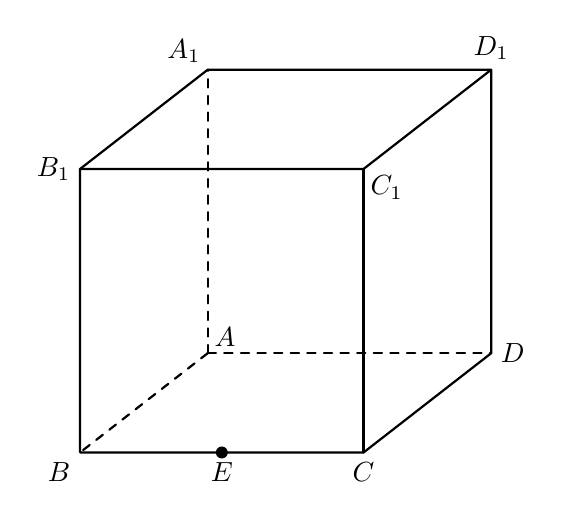
\begin{tikzpicture}[scale=1.8, line join=round, line cap=round, >=stealth]
  % 顶点坐标设定（正方体斜二测标准投影）
  \coordinate (B) at (0, 0);
  \coordinate (C) at (2.0, 0);
  \coordinate (A) at (0.9, 0.7);
  \coordinate (D) at (2.9, 0.7);

  \coordinate (B1) at (0, 2.0);
  \coordinate (C1) at (2.0, 2.0);
  \coordinate (A1) at (0.9, 2.7);
  \coordinate (D1) at (2.9, 2.7);

  % 棱 BC 中点 E
  \coordinate (E) at (1.0, 0);

  % 虚线部分（后侧与内部不可见棱）
  \draw[dashed, thick] (A) -- (B);
  \draw[dashed, thick] (A) -- (D);
  \draw[dashed, thick] (A) -- (A1);

  % 实线部分（外轮廓与可见棱）
  \draw[thick] (B) -- (C) -- (D) -- (D1) -- (A1) -- (B1) -- cycle;
  \draw[thick] (B1) -- (C1) -- (D1);
  \draw[thick] (C) -- (C1);

  % 关键点标记
  \fill (E) circle (1.2pt);

  % 顶点标注
  \node[below left] at (B) {$B$};
  \node[below] at (C) {$C$};
  \node[right] at (D) {$D$};
  \node[above right=-1pt] at (A) {$A$};

  \node[left] at (B1) {$B_1$};
  \node[below right=-1pt] at (C1) {$C_1$};
  \node[above] at (D1) {$D_1$};
  \node[above left=-1pt] at (A1) {$A_1$};

  \node[below] at (E) {$E$};
\end{tikzpicture}
\end{center}
\nopagebreak[4]
\Needspace{4\baselineskip}
\textbf{解析}
\nopagebreak[4]
\begin{center}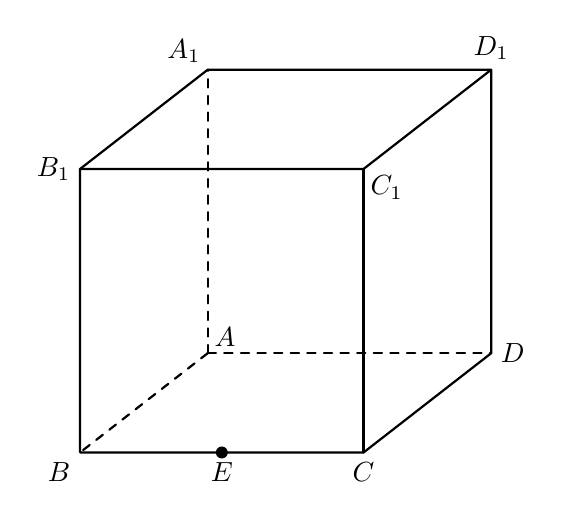
\begin{tikzpicture}[scale=1.8, line join=round, line cap=round, >=stealth]
  % 顶点坐标设定（正方体斜二测标准投影）
  \coordinate (B) at (0, 0);
  \coordinate (C) at (2.0, 0);
  \coordinate (A) at (0.9, 0.7);
  \coordinate (D) at (2.9, 0.7);

  \coordinate (B1) at (0, 2.0);
  \coordinate (C1) at (2.0, 2.0);
  \coordinate (A1) at (0.9, 2.7);
  \coordinate (D1) at (2.9, 2.7);

  % 棱 BC 中点 E
  \coordinate (E) at (1.0, 0);

  % 虚线部分（后侧与内部不可见棱）
  \draw[dashed, thick] (A) -- (B);
  \draw[dashed, thick] (A) -- (D);
  \draw[dashed, thick] (A) -- (A1);

  % 实线部分（外轮廓与可见棱）
  \draw[thick] (B) -- (C) -- (D) -- (D1) -- (A1) -- (B1) -- cycle;
  \draw[thick] (B1) -- (C1) -- (D1);
  \draw[thick] (C) -- (C1);

  % 关键点标记
  \fill (E) circle (1.2pt);

  % 顶点标注
  \node[below left] at (B) {$B$};
  \node[below] at (C) {$C$};
  \node[right] at (D) {$D$};
  \node[above right=-1pt] at (A) {$A$};

  \node[left] at (B1) {$B_1$};
  \node[below right=-1pt] at (C1) {$C_1$};
  \node[above] at (D1) {$D_1$};
  \node[above left=-1pt] at (A1) {$A_1$};

  \node[below] at (E) {$E$};
\end{tikzpicture}
\end{center}
\nopagebreak[4]
以点 $D$ 为坐标原点，以射线 $DA$ 为 $x$ 轴正方向，以射线 $DC$ 为 $y$ 轴正方向，以射线 $DD_1$ 为 $z$ 轴正方向建立空间直角坐标系 $D - xyz$．
\Needspace{5\baselineskip}
正方体的棱长为 $1$，各关键点坐标为：
\nopagebreak[4]
\[
D(0, 0, 0), \quad A(1, 0, 0), \quad B(1, 1, 0), \quad C(0, 1, 0),
\]
\nopagebreak[4]
\[
D_1(0, 0, 1), \quad A_1(1, 0, 1), \quad B_1(1, 1, 1), \quad C_1(0, 1, 1).
\]
点 $E$ 是棱 $BC$ 的中点，故 $E\left(\dfrac{1}{2}, 1, 0\right)$．
点 $F$ 是棱 $CD$ 上的动点，设 $F(0, \lambda, 0)$，其中 $0 \leqslant \lambda \leqslant 1$．

\Needspace{5\baselineskip}
（1）连接 $D_1E$，其方向向量为：
\nopagebreak[4]
\[
\overrightarrow{D_1E} = E - D_1 = \left(\frac{1}{2}, 1, -1\right).
\]
\Needspace{5\baselineskip}
平面 $AB_1F$ 内包含向量 $\overrightarrow{AB_1}$ 与 $\overrightarrow{AF}$：
\nopagebreak[4]
\[
\overrightarrow{AB_1} = B_1 - A = (0, 1, 1), \quad \overrightarrow{AF} = F - A = (-1, \lambda, 0).
\]
\Needspace{5\baselineskip}
计算 $\overrightarrow{D_1E} \cdot \overrightarrow{AB_1}$：
\nopagebreak[4]
\[
\overrightarrow{D_1E} \cdot \overrightarrow{AB_1} = \frac{1}{2} \times 0 + 1 \times 1 + (-1) \times 1 = 0.
\]
这说明无论动点 $F$ 在何位置，直线 $D_1E$ 始终与平面内的直线 $AB_1$ 垂直．
\Needspace{5\baselineskip}
要使 $D_1E \perp \text{\text{平面} } AB_1F$，只需 $D_1E \perp AF$，即：
\nopagebreak[4]
\[
\overrightarrow{D_1E} \cdot \overrightarrow{AF} = \frac{1}{2} \times (-1) + 1 \times \lambda + (-1) \times 0 = -\frac{1}{2} + \lambda = 0 \implies \lambda = \frac{1}{2}.
\]
因为 $\lambda = \dfrac{1}{2}$，点 $F$ 的坐标为 $\left(0, \dfrac{1}{2}, 0\right)$，恰好是棱 $CD$ 的中点．
因此，当点 $F$ 是棱 $CD$ 的中点时，$D_1E \perp \text{\text{平面} } AB_1F$．

（2）当 $D_1E \perp \text{\text{平面} } AB_1F$ 时，$F$ 为棱 $CD$ 的中点，坐标为 $F\left(0, \dfrac{1}{2}, 0\right)$．
二面角 $C_1 - EF - A$ 的棱为直线 $EF$：
\begin{itemize}
\item 半平面 $AEF$ 处于正方体底面 $ABCD$ 所在平面，其一个向上的法向量为 $\vec{n}_1 = (0, 0, 1)$；
\item 求解半平面 $C_1EF$ 的法向量 $\vec{n}_2$：
\end{itemize}
\Needspace{5\baselineskip}
  在平面 $C_1EF$ 内，有向量：
\nopagebreak[4]
\[
\overrightarrow{FE} = E - F = \left(\frac{1}{2}, \frac{1}{2}, 0\right), \quad \overrightarrow{FC_1} = C_1 - F = \left(0, \frac{1}{2}, 1\right).
\]
\Needspace{5\baselineskip}
  设 $\vec{n}_2 = (x, y, z)$，由法向量垂直于平面内两不共线向量：
\nopagebreak[4]
\[
\begin{cases}
\vec{n}_2 \cdot \overrightarrow{FE} = \dfrac{1}{2}x + \dfrac{1}{2}y = 0 \implies y = -x, \\
\vec{n}_2 \cdot \overrightarrow{FC_1} = \dfrac{1}{2}y + z = 0 \implies z = -\dfrac{1}{2}y = \dfrac{1}{2}x.
\end{cases}
\]
  取 $x = 2$，则 $y = -2, z = 1$，得平面 $C_1EF$ 的一个法向量为 $\vec{n}_2 = (2, -2, 1)$．
\Needspace{5\baselineskip}
计算两法向量夹角余弦的绝对值：
\nopagebreak[4]
\[
|\cos\langle \vec{n}_1, \vec{n}_2 \rangle| = \frac{|\vec{n}_1 \cdot \vec{n}_2|}{|\vec{n}_1||\vec{n}_2|} = \frac{|1|}{1 \times \sqrt{2^2 + (-2)^2 + 1^2}} = \frac{1}{3}.
\]
观察空间几何方位：棱 $EF$ 将底面划分为包含顶点 $C$ 的等腰直角三角形区域与包含顶点 $A$ 的五边形区域；顶点 $C_1$ 位于点 $C$ 的正上方，因此半平面 $C_1EF$ 与半平面 $AEF$ 所构成的二面角为钝角．
因此，二面角 $C_1 - EF - A$ 的大小为 $\arccos\left(-\dfrac{1}{3}\right)$（或 $\pi - \arccos\dfrac{1}{3}$）．

\gkanswer{答案：（1）点 $F$ 为棱 $CD$ 的中点；（2）$\arccos\left(-\dfrac{1}{3}\right)$（或 $\pi - \arccos\dfrac{1}{3}$）}

\end{answer}
\begin{answer}
\gksolhead{19}{}

\textbf{题目}：

如图，在 $\mathrm{Rt}\triangle ABC$ 中，已知 $BC = a$，若长为 $2a$ 的线段 $PQ$ 以点 $A$ 为中点，问 $\vec{PQ}$ 与 $\vec{BC}$ 的夹角 $\theta$ 取何值时 $\vec{BP} \cdot \vec{CQ}$ 的值最大？并求出这个最大值．
\nopagebreak[4]
\begin{center}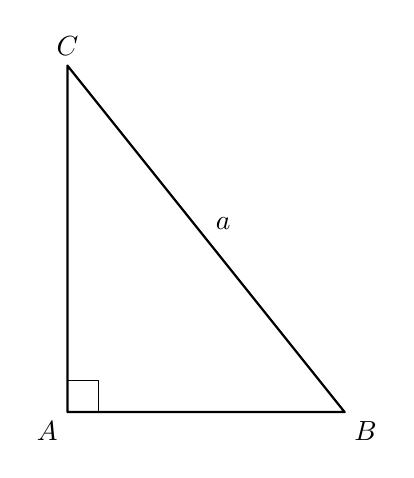
\begin{tikzpicture}[scale=2.2, line join=round, line cap=round]
  \coordinate (A) at (0, 0);
  \coordinate (B) at (1.6, 0);
  \coordinate (C) at (0, 2.0);

  % 绘制直角三角形
  \draw[thick] (A) -- (B) -- (C) -- cycle;

  % 直角标记
  \draw[thin] (0, 0.18) -- (0.18, 0.18) -- (0.18, 0);

  % 顶点与边长标注
  \node[below left] at (A) {$A$};
  \node[below right] at (B) {$B$};
  \node[above] at (C) {$C$};
  \node[above right] at (0.8, 1.0) {$a$};
\end{tikzpicture}
\end{center}
\nopagebreak[4]
\Needspace{4\baselineskip}
\textbf{解析}
\nopagebreak[4]
\begin{center}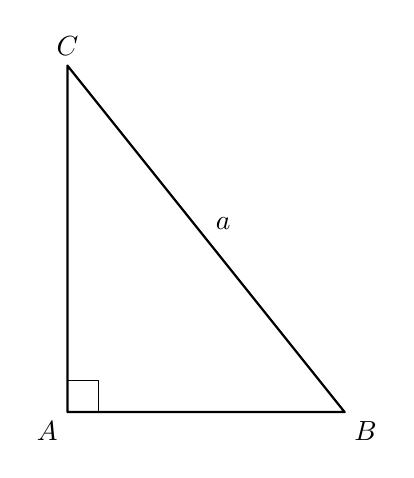
\begin{tikzpicture}[scale=2.2, line join=round, line cap=round]
  \coordinate (A) at (0, 0);
  \coordinate (B) at (1.6, 0);
  \coordinate (C) at (0, 2.0);

  % 绘制直角三角形
  \draw[thick] (A) -- (B) -- (C) -- cycle;

  % 直角标记
  \draw[thin] (0, 0.18) -- (0.18, 0.18) -- (0.18, 0);

  % 顶点与边长标注
  \node[below left] at (A) {$A$};
  \node[below right] at (B) {$B$};
  \node[above] at (C) {$C$};
  \node[above right] at (0.8, 1.0) {$a$};
\end{tikzpicture}
\end{center}
\nopagebreak[4]
在 $\mathrm{Rt}\triangle ABC$ 中，已知 $BC = a$，$A$ 为直角顶点，故 $AB \perp AC$，即 $\overrightarrow{BA} \cdot \overrightarrow{CA} = 0$．
\Needspace{5\baselineskip}
因为点 $A$ 是线段 $PQ$ 的中点，且线段长 $|PQ| = 2a$，所以：
\nopagebreak[4]
\[
|AP| = |AQ| = a, \quad \overrightarrow{AQ} = -\overrightarrow{AP}.
\]
\Needspace{5\baselineskip}
利用向量的三角形法则，将 $\overrightarrow{BP}$ 与 $\overrightarrow{CQ}$ 用经过点 $A$ 的向量表示：
\nopagebreak[4]
\[
\overrightarrow{BP} = \overrightarrow{BA} + \overrightarrow{AP},
\]
\nopagebreak[4]
\[
\overrightarrow{CQ} = \overrightarrow{CA} + \overrightarrow{AQ} = \overrightarrow{CA} - \overrightarrow{AP}.
\]
\Needspace{5\baselineskip}
计算数量积 $\overrightarrow{BP} \cdot \overrightarrow{CQ}$：
\nopagebreak[4]
\[
\begin{aligned}
\overrightarrow{BP} \cdot \overrightarrow{CQ} &= (\overrightarrow{BA} + \overrightarrow{AP}) \cdot (\overrightarrow{CA} - \overrightarrow{AP}) \\
&= \overrightarrow{BA} \cdot \overrightarrow{CA} - \overrightarrow{BA} \cdot \overrightarrow{AP} + \overrightarrow{AP} \cdot \overrightarrow{CA} - |\overrightarrow{AP}|^2.
\end{aligned}
\]
由于 $AB \perp AC$，$\overrightarrow{BA} \cdot \overrightarrow{CA} = 0$；
又 $|\overrightarrow{AP}| = a$，故 $|\overrightarrow{AP}|^2 = a^2$．
\Needspace{5\baselineskip}
整理得：
\nopagebreak[4]
\[
\overrightarrow{BP} \cdot \overrightarrow{CQ} = -a^2 - \overrightarrow{AP} \cdot (\overrightarrow{BA} - \overrightarrow{CA}) = -a^2 - \overrightarrow{AP} \cdot \overrightarrow{BC}.
\]
因为点 $A$ 是线段 $PQ$ 的中点，所以 $\overrightarrow{PQ} = 2\overrightarrow{AQ} = -2\overrightarrow{AP}$，即 $\overrightarrow{AP} = -\dfrac{1}{2}\overrightarrow{PQ}$．
\Needspace{5\baselineskip}
代入上式得：
\nopagebreak[4]
\[
\overrightarrow{BP} \cdot \overrightarrow{CQ} = -a^2 - \left(-\frac{1}{2}\overrightarrow{PQ}\right) \cdot \overrightarrow{BC} = -a^2 + \frac{1}{2}\overrightarrow{PQ} \cdot \overrightarrow{BC}.
\]
\Needspace{5\baselineskip}
已知 $|\overrightarrow{PQ}| = 2a$，$|\overrightarrow{BC}| = a$，设 $\overrightarrow{PQ}$ 与 $\overrightarrow{BC}$ 的夹角为 $\theta$（$\theta \in [0, \pi]$）：
\nopagebreak[4]
\[
\overrightarrow{PQ} \cdot \overrightarrow{BC} = |\overrightarrow{PQ}||\overrightarrow{BC}|\cos\theta = 2a \times a \times \cos\theta = 2a^2 \cos\theta.
\]
\Needspace{5\baselineskip}
因此：
\nopagebreak[4]
\[
\overrightarrow{BP} \cdot \overrightarrow{CQ} = -a^2 + \frac{1}{2}(2a^2 \cos\theta) = a^2(\cos\theta - 1).
\]
因为 $\theta \in [0, \pi]$，余弦函数满足 $\cos\theta \leqslant 1$，
当且仅当 $\theta = 0$（即向量 $\overrightarrow{PQ}$ 与 $\overrightarrow{BC}$ 同向共线）时，$\cos\theta$ 取得最大值 $1$．
\Needspace{5\baselineskip}
此时 $\overrightarrow{BP} \cdot \overrightarrow{CQ}$ 取得最大值：
\nopagebreak[4]
\[
\max \left(\overrightarrow{BP} \cdot \overrightarrow{CQ}\right) = a^2(1 - 1) = 0.
\]
综上所述，当 $\theta = 0$ 时，$\overrightarrow{BP} \cdot \overrightarrow{CQ}$ 的值最大，最大值为 $0$．

\gkanswer{答案：当 $\theta = 0$ 时，$\vec{BP} \cdot \vec{CQ}$ 的值最大，最大值为 $0$}

\end{answer}
\begin{answer}
\gksolhead{20}{}

\textbf{题目}：

直线 $l: y = kx + 1$ 与双曲线 $C: 2x^2 - y^2 = 1$ 的右支交于不同的两点 $A$、$B$．

（1）求实数 $k$ 的取值范围；

（2）是否存在实数 $k$，使得以线段 $AB$ 为直径的圆经过双曲线 $C$ 的右焦点 $F$？若存在，求出 $k$ 的值．若不存在，说明理由．

\Needspace{4\baselineskip}
\textbf{解析}
\nopagebreak[4]
\begin{center}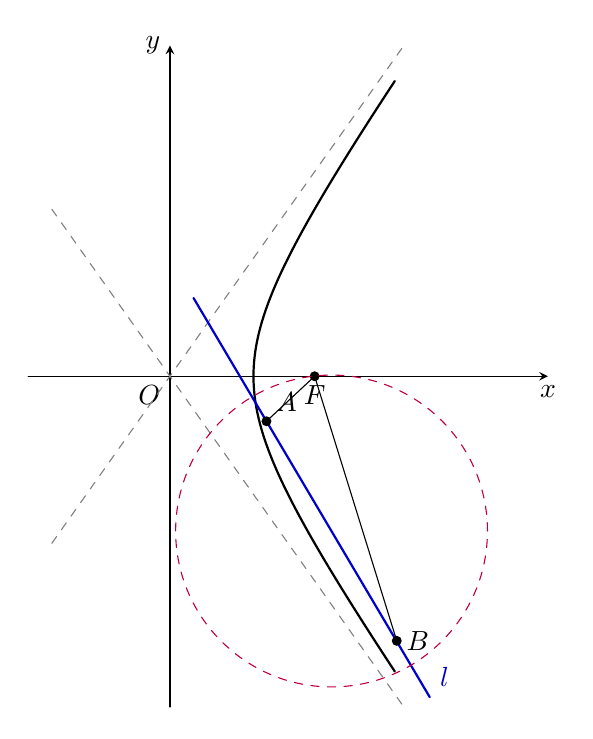
\begin{tikzpicture}[scale=1.5, >=stealth, line cap=round, line join=round]
  % 坐标轴
  \draw[->] (-1.2, 0) -- (3.2, 0) node[below] {$x$};
  \draw[->] (0, -2.8) -- (0, 2.8) node[left] {$y$};
  \node[below left] at (0, 0) {$O$};

  % 渐近线
  \draw[dashed, thin, gray] (-1.0, -1.414) -- (2.0, 2.828);
  \draw[dashed, thin, gray] (-1.0, 1.414) -- (2.0, -2.828);

  % 双曲线右支 2x^2 - y^2 = 1 => x = sqrt((1 + y^2)/2)
  \draw[thick, smooth, domain=-2.5:2.5, samples=60] 
    plot ({sqrt((1 + \x*\x)/2)}, \x);

  % 焦点 F(sqrt(6)/2, 0) ≈ (1.225, 0)
  \coordinate (F) at (1.2247, 0);
  \fill (F) circle (1.2pt) node[below] {$F$};

  % 直线 y = kx + 1，k = -(6 + sqrt(6))/5 ≈ -1.6899
  \coordinate (A) at (0.817, -0.381);
  \coordinate (B) at (1.92, -2.24);
  \draw[domain=0.2:2.2, smooth, thick, blue!80!black] 
    plot (\x, {-1.6899*\x + 1}) node[above right] {$l$};

  \fill (A) circle (1.2pt) node[above right] {$A$};
  \fill (B) circle (1.2pt) node[right] {$B$};

  % 直径圆中心与圆
  \coordinate (M) at (1.368, -1.31);
  \draw[dashed, thin, purple] (M) circle (1.32);

  \draw[thin] (A) -- (F) -- (B);
\end{tikzpicture}
\end{center}
\nopagebreak[4]
（1）直线方程为 $l: y = kx + 1$，双曲线方程为 $C: 2x^2 - y^2 = 1$（即 $\dfrac{x^2}{1/2} - \dfrac{y^2}{1} = 1$）．
\Needspace{5\baselineskip}
将直线方程代入双曲线方程：
\nopagebreak[4]
\[
2x^2 - (kx + 1)^2 = 1 \implies (2 - k^2)x^2 - 2kx - 2 = 0.
\]
设直线与双曲线的两个不同交点为 $A(x_1, y_1), B(x_2, y_2)$．
由题意，直线与双曲线的右支交于不同的两点，必须且只需满足以下条件：
① 二次项系数不为零：$2 - k^2 \neq 0$，即 $k \neq \pm \sqrt{2}$；
\Needspace{5\baselineskip}
② 判别式大于零：
\nopagebreak[4]
\[
\Delta = (-2k)^2 - 4(2 - k^2)(-2) = 4k^2 + 8(2 - k^2) = 16 - 4k^2 > 0 \implies k^2 < 4 \implies -2 < k < 2;
\]
\Needspace{5\baselineskip}
③ 两交点均在右支上，即 $x_1 > \dfrac{\sqrt{2}}{2}$ 且 $x_2 > \dfrac{\sqrt{2}}{2}$，由韦达定理：
\nopagebreak[4]
\[
x_1 + x_2 = \frac{2k}{2 - k^2} > 0, \quad x_1 x_2 = \frac{-2}{2 - k^2} > 0.
\]
   由 $x_1 x_2 = \dfrac{-2}{2 - k^2} > 0$ 得 $2 - k^2 < 0 \implies k^2 > 2$；
   再由 $x_1 + x_2 = \dfrac{2k}{2 - k^2} > 0$，因分母 $2 - k^2 < 0$，必有分子 $2k < 0 \implies k < 0$．
\Needspace{5\baselineskip}
结合 $k^2 < 4$ 与 $k^2 > 2, k < 0$，解得：
\nopagebreak[4]
\[
-\sqrt{4} < k < -\sqrt{2} \implies -2 < k < -\sqrt{2}.
\]
此时双曲线右顶点为 $\left(\dfrac{\sqrt{2}}{2}, 0\right)$，方程根满足 $x_1 x_2 = \dfrac{2}{k^2 - 2} > 1 > \dfrac{1}{2}$，两根均大于 $\dfrac{\sqrt{2}}{2}$，两交点确实均落在右支上．
因此，实数 $k$ 的取值范围为 $(-2, -\sqrt{2})$．

（2）双曲线 $C: \dfrac{x^2}{1/2} - \dfrac{y^2}{1} = 1$ 的半焦距为 $c = \sqrt{a^2 + b^2} = \sqrt{\dfrac{1}{2} + 1} = \dfrac{\sqrt{6}}{2}$．
右焦点为 $F\left(\dfrac{\sqrt{6}}{2}, 0\right)$．
以线段 $AB$ 为直径的圆经过点 $F$，等价于 $\angle AFB = 90^\circ$，即 $\overrightarrow{FA} \cdot \overrightarrow{FB} = 0$．
\Needspace{5\baselineskip}
因为点 $A(x_1, y_1), B(x_2, y_2)$ 在直线 $y = kx + 1$ 上，所以：
\nopagebreak[4]
\[
\overrightarrow{FA} = \left(x_1 - \frac{\sqrt{6}}{2}, kx_1 + 1\right), \quad \overrightarrow{FB} = \left(x_2 - \frac{\sqrt{6}}{2}, kx_2 + 1\right).
\]
\Needspace{5\baselineskip}
计算数量积：
\nopagebreak[4]
\[
\begin{aligned}
\overrightarrow{FA} \cdot \overrightarrow{FB} &= \left(x_1 - \frac{\sqrt{6}}{2}\right)\left(x_2 - \frac{\sqrt{6}}{2}\right) + (kx_1 + 1)(kx_2 + 1) \\
&= x_1 x_2 - \frac{\sqrt{6}}{2}(x_1 + x_2) + \frac{3}{2} + k^2 x_1 x_2 + k(x_1 + x_2) + 1 \\
&= (k^2 + 1)x_1 x_2 + \left(k - \frac{\sqrt{6}}{2}\right)(x_1 + x_2) + \frac{5}{2}.
\end{aligned}
\]
\Needspace{5\baselineskip}
将韦达定理 $x_1 + x_2 = \dfrac{2k}{2 - k^2}, x_1 x_2 = \dfrac{-2}{2 - k^2}$ 代入，并令数量积为 $0$：
\nopagebreak[4]
\[
(k^2 + 1)\left(\frac{-2}{2 - k^2}\right) + \left(k - \frac{\sqrt{6}}{2}\right)\left(\frac{2k}{2 - k^2}\right) + \frac{5}{2} = 0.
\]
\Needspace{5\baselineskip}
两边同乘以 $2(2 - k^2)$：
\nopagebreak[4]
\[
-4(k^2 + 1) + 4k\left(k - \frac{\sqrt{6}}{2}\right) + 5(2 - k^2) = 0.
\]
\Needspace{5\baselineskip}
展开整理：
\nopagebreak[4]
\[
-4k^2 - 4 + 4k^2 - 2\sqrt{6}k + 10 - 5k^2 = 0 \implies 5k^2 + 2\sqrt{6}k - 6 = 0.
\]
\Needspace{5\baselineskip}
解此一元二次方程，判别式 $\Delta_k = (2\sqrt{6})^2 - 4 \times 5 \times (-6) = 24 + 120 = 144 = 12^2$：
\nopagebreak[4]
\[
k = \frac{-2\sqrt{6} \pm 12}{10} = \frac{-\sqrt{6} \pm 6}{5}.
\]
检验两个实数根：
\begin{itemize}
\item $k_1 = \dfrac{6 - \sqrt{6}}{5} > 0$，不满足第（1）问中 $k \in (-2, -\sqrt{2})$ 的要求，舍去；
\item $k_2 = \dfrac{-6 - \sqrt{6}}{5} = -\dfrac{6 + \sqrt{6}}{5}$．
\end{itemize}
\Needspace{5\baselineskip}
因为 $2.449 < \sqrt{6} < 2.450$，所以 $8.449 < 6 + \sqrt{6} < 8.450$，
\nopagebreak[4]
\[
-1.690 < -\frac{6 + \sqrt{6}}{5} < -1.689.
\]
而 $-2 < -1.690$ 且 $-1.689 < -\sqrt{2} \approx -1.414$，因此 $k_2 \in (-2, -\sqrt{2})$ 成立．
综上所述，存在实数 $k = -\dfrac{6 + \sqrt{6}}{5}$，使得以线段 $AB$ 为直径的圆经过双曲线 $C$ 的右焦点 $F$．

\gkanswer{答案：（1）$(-2, -\sqrt{2})$；（2）存在，$k = -\dfrac{6 + \sqrt{6}}{5}$}

\end{answer}
\begin{answer}
\gksolhead{21}{}

\textbf{题目}：

某突发事件，在不采取任何预防措施的情况下发生的概率为 $0.3$；一旦发生，将造成 $400$ 万元的损失．现有甲、乙两种相互独立的预防措施可供采用．单独采用甲、乙预防措施所需的费用分别为 $45$ 万元和 $30$ 万元，采用相应预防措施后此突发事件不发生的概率分别是 $0.9$ 和 $0.85$．若预防方案允许甲、乙两种预防措施单独采用、联合采用或不采用，请确定预防方案使总费用最少．

注：总费用 = 采取预防措施的费用 + 发生突发事件损失的期望值．

\Needspace{4\baselineskip}
\textbf{解析}

设突发事件为事件 $E$．若不采取任何预防措施，$E$ 发生的概率为 $P(E) = 0.3$；一旦发生造成的损失为 $400$ 万元．
根据题意，预防方案允许甲、乙两种措施单独采用、联合采用或不采用，共有以下 $4$ 种可供选择的方案：

1. \textbf{方案 1：不采取任何预防措施}
\begin{itemize}
\item 措施费用为 $C_1 = 0$ 万元；
\item 突发事件发生的概率为 $P_1 = 0.3$；
\item 损失期望值为 $E_1 = 400 \times 0.3 = 120$ 万元；
\item 总费用为 $T_1 = 0 + 120 = 120$ 万元．
\end{itemize}

2. \textbf{方案 2：单独采用预防措施乙}
\begin{itemize}
\item 措施费用为 $C_2 = 30$ 万元；
\item 采用乙措施后，突发事件不发生的概率为 $0.85$，故事件发生的概率为 $P_2 = 1 - 0.85 = 0.15$；
\item 损失期望值为 $E_2 = 400 \times 0.15 = 60$ 万元；
\item 总费用为 $T_2 = 30 + 60 = 90$ 万元．
\end{itemize}

3. \textbf{方案 3：单独采用预防措施甲}
\begin{itemize}
\item 措施费用为 $C_3 = 45$ 万元；
\item 采用甲措施后，突发事件不发生的概率为 $0.9$，故事件发生的概率为 $P_3 = 1 - 0.9 = 0.1$；
\item 损失期望值为 $E_3 = 400 \times 0.1 = 40$ 万元；
\item 总费用为 $T_3 = 45 + 40 = 85$ 万元．
\end{itemize}

4. \textbf{方案 4：联合采用甲、乙两种预防措施}
\begin{itemize}
\item 措施费用为 $C_4 = 45 + 30 = 75$ 万元；
\item 因为甲、乙两种预防措施相互独立，联合采用时，突发事件发生当且仅当甲措施未能阻止且乙措施也未能阻止．
\end{itemize}
\Needspace{5\baselineskip}
     因此，事件发生的概率为两措施均失效的概率：
\nopagebreak[4]
\[
P_4 = (1 - 0.9) \times (1 - 0.85) = 0.1 \times 0.15 = 0.015.
\]
\begin{itemize}
\item 损失期望值为 $E_4 = 400 \times 0.015 = 6$ 万元；
\item 总费用为 $T_4 = 75 + 6 = 81$ 万元．
\end{itemize}

\Needspace{5\baselineskip}
对比以上各方案的总费用：
\nopagebreak[4]
\[
T_4 = 81 < T_3 = 85 < T_2 = 90 < T_1 = 120.
\]
因此，最少总费用为 $81$ 万元，最优预防方案是联合采用甲、乙两种预防措施．

\gkanswer{答案：联合采用甲、乙两种预防措施使总费用最少，最少总费用为 $81$ 万元}

\end{answer}
\begin{answer}
\gksolhead{22}{}

\textbf{题目}：

已知 $a > 0$，数列 $\{a_n\}$ 满足 $a_1 = a$，$a_{n+1} = a + \dfrac{1}{a_n}$，$n = 1, 2, \cdots$．

（1）已知数列 $\{a_n\}$ 极限存在且大于零，求 $A = \lim_{n\to\infty} a_n$（将 $A$ 用 $a$ 表示）；

（2）设 $b_n = a_n - A$，$n = 1, 2, \cdots$，证明：$b_{n+1} = -\dfrac{b_n}{A(b_n + A)}$；

（3）若 $|b_n| \leqslant \dfrac{1}{2^n}$ 对 $n = 1, 2, \cdots$ 都成立，求 $a$ 的取值范围．

\Needspace{4\baselineskip}
\textbf{解析}

\Needspace{5\baselineskip}
（1）已知数列 $\{a_n\}$ 满足递推关系：
\nopagebreak[4]
\[
a_1 = a > 0, \quad a_{n+1} = a + \frac{1}{a_n}, \quad (n = 1, 2, \cdots).
\]
已知数列极限 $A = \lim_{n\to\infty} a_n$ 存在且 $A > 0$．
\Needspace{5\baselineskip}
对递推式两边取极限：
\nopagebreak[4]
\[
\lim_{n\to\infty} a_{n+1} = a + \frac{1}{\lim_{n\to\infty} a_n} \implies A = a + \frac{1}{A}.
\]
\Needspace{5\baselineskip}
方程两边同乘以 $A$ 得：
\nopagebreak[4]
\[
A^2 - aA - 1 = 0.
\]
\Needspace{5\baselineskip}
解此一元二次方程：
\nopagebreak[4]
\[
A = \frac{a \pm \sqrt{a^2 + 4}}{2}.
\]
因为 $a > 0$ 且极限 $A > 0$，而 $\sqrt{a^2 + 4} > a$，若取负号则 $A < 0$，不合题意，故舍去负根．
\Needspace{5\baselineskip}
因此：
\nopagebreak[4]
\[
A = \frac{a + \sqrt{a^2 + 4}}{2}.
\]

（2）证明：由 $A = a + \dfrac{1}{A}$，可得 $a - A = -\dfrac{1}{A}$．
设 $b_n = a_n - A$，则 $a_n = b_n + A$，$a_{n+1} = b_{n+1} + A$．
\Needspace{5\baselineskip}
代入原数列的递推关系式：
\nopagebreak[4]
\[
b_{n+1} + A = a + \frac{1}{b_n + A} \implies b_{n+1} = a - A + \frac{1}{b_n + A}.
\]
\Needspace{5\baselineskip}
将 $a - A = -\dfrac{1}{A}$ 代入上式并通分：
\nopagebreak[4]
\[
b_{n+1} = -\frac{1}{A} + \frac{1}{b_n + A} = \frac{-(b_n + A) + A}{A(b_n + A)} = -\frac{b_n}{A(b_n + A)}.
\]
命题得证．

\Needspace{5\baselineskip}
（3）由（2）的递推式，考察首项 $b_1$：
\nopagebreak[4]
\[
b_1 = a_1 - A = a - A = -\frac{1}{A}.
\]
\Needspace{5\baselineskip}
要使 $|b_n| \leqslant \dfrac{1}{2^n}$ 对所有 $n = 1, 2, \cdots$ 都成立，必须对 $n = 1$ 成立，即：
\nopagebreak[4]
\[
|b_1| = \left|-\frac{1}{A}\right| = \frac{1}{A} \leqslant \frac{1}{2} \implies A \geqslant 2.
\]
\Needspace{5\baselineskip}
将 $A = \dfrac{a + \sqrt{a^2 + 4}}{2}$ 代入 $A \geqslant 2$：
\nopagebreak[4]
\[
\frac{a + \sqrt{a^2 + 4}}{2} \geqslant 2 \iff \sqrt{a^2 + 4} \geqslant 4 - a.
\]
\begin{itemize}
\item 若 $a \geqslant 4$，不等式显然成立；
\item 若 $0 < a < 4$，两边平方得：
\end{itemize}
\nopagebreak[4]
\[
a^2 + 4 \geqslant 16 - 8a + a^2 \implies 8a \geqslant 12 \implies a \geqslant \frac{3}{2}.
\]
因此 $A \geqslant 2 \iff a \geqslant \dfrac{3}{2}$．

下面证明当 $a \geqslant \dfrac{3}{2}$ 时，$|b_n| \leqslant \dfrac{1}{2^n}$ 对所有正整数 $n$ 恒成立：
\Needspace{5\baselineskip}
因为 $a_1 = a \geqslant \dfrac{3}{2}$，且对任意 $n \geqslant 1$：
\nopagebreak[4]
\[
a_{n+1} = a + \frac{1}{a_n} > a \geqslant \frac{3}{2}.
\]
由数学归纳法可知，对任意 $n \geqslant 1$，均有 $a_n \geqslant a$．
\Needspace{5\baselineskip}
又因为 $A \geqslant 2$，$a = A - \dfrac{1}{A}$，所以：
\nopagebreak[4]
\[
A(b_n + A) = A a_n \geqslant A a = A\left(A - \frac{1}{A}\right) = A^2 - 1 \geqslant 2^2 - 1 = 3 > 2.
\]
\Needspace{5\baselineskip}
由（2）的递推关系，取绝对值：
\nopagebreak[4]
\[
|b_{n+1}| = \frac{|b_n|}{A(b_n + A)} = \frac{|b_n|}{A a_n} \leqslant \frac{|b_n|}{3} \leqslant \frac{1}{2}|b_n|.
\]
\Needspace{5\baselineskip}
由此递推得：
\nopagebreak[4]
\[
|b_n| \leqslant \left(\frac{1}{2}\right)^{n-1} |b_1| = \left(\frac{1}{2}\right)^{n-1} \frac{1}{A} \leqslant \left(\frac{1}{2}\right)^{n-1} \cdot \frac{1}{2} = \frac{1}{2^n}.
\]
因此，$|b_n| \leqslant \dfrac{1}{2^n}$ 对所有 $n = 1, 2, \cdots$ 均成立．
综上所述，$a$ 的取值范围为 $\left[\dfrac{3}{2}, +\infty\right)$（即 $a \geqslant \dfrac{3}{2}$）．

\gkanswer{答案：（1）$A = \dfrac{a + \sqrt{a^2 + 4}}{2}$；（2）证明见解析；（3）$a \geqslant \dfrac{3}{2}$（或 $\left[\dfrac{3}{2}, +\infty\right)$）}

\end{answer}